\documentclass[
    pagesize,%         put paper size information into document (for ps and pdf!)
    a4paper,%          use a5paper for ISO A5; use a4paper for ISO A4
            %          adapt also pdf paper size!
%    BCOR12mm,%         set extra margin for book fixation
%    DIV11,%            set DIV for good linewidth explicitly
%    DIVcalc,%            typearea has to calculate DIV for good linewidth
    headsepline,%      use headinclude also! (see M. Kohm)
    footsepline,%      use footinclude also! (see M. Kohm)
    headinclude,%      count head to text body (not to margin) 
    footinclude,%      count foot to text body (not to margin) 
    bibtotoc,%         write bibliography-chapter to table of contents
%    idxtotoc,           % Stichwortverzeichnis ebenso
%    liststotoc,%       abbildungs- und tabellenverzeichnis ebenso
    cleardoubleplain,% \cleardoublepage generates pages with pagestyle plain
    tablecaptionabove,% setzt tabel caption besser ab 
%    final%            final version
%    draft%            draft version
]{scrreprt}



\usepackage[latin9]{inputenc}
\usepackage[english]{babel}
\usepackage[T1]{fontenc}

\usepackage{graphicx}
\usepackage{amsmath}
\usepackage{booktabs}
\usepackage{textcomp}
\usepackage{multirow}
\usepackage{color}
\usepackage{babelbib}
\usepackage{setspace}
\usepackage{booktabs}
\usepackage{gensymb}
\usepackage{pdflscape}
\usepackage{multirow}
\usepackage[table]{xcolor}
\usepackage{longtable}
\usepackage[font={small,sf},format=plain,labelfont={bf,up}]{caption} %im text \textbf könnte raus
\usepackage{adjustbox}
\usepackage{etoolbox}
\usepackage[master,institut]{zfibmcover}        % load cover
\usepackage[sort]{natbib} % base bib style


% The following package makes code look a little nicer, but it may not be present on all systems.
\IfFileExists{cmtt.sty}{\usepackage[override]{cmtt}}{}% better typewriter font
% \usepackage{ae}      % erzeuge lesbare Schriften in pdf (almost european
                       % font)




% ---------------------
% some default settings
% ---------------------

% caption font settings
\setkomafont{captionlabel}{\usekomafont{section}\footnotesize}
\setkomafont{caption}{\normalfont\itshape\footnotesize}

% Keine Serifenlose fuer description-Umgebungen
%
\renewcommand{\descfont}{\normalfont\bfseries}

% serifenlose und kleinere Schrift in Kopf und Fuss
\setkomafont{pagehead}{\normalcolor\sffamily\small}% what about \itshape?

\raggedbottom % Tanzender Fuss, tanzende fussnoten



\renewcommand{\cite}{\citep*}% change citation default command
\newcommand{\cites}{\citet*}% use for citation in sentence

\bibpunct{(}{)}{;}{a}{}{,~} % configure citation style

\bibfont{\small} % smaller font for bibliography


\usepackage[NewCommands]{ragged2e} % overwrite old commands with new ones
\renewcommand*{\raggedsection}{\RaggedRight} % ragged right headings

% we want a flushleft bibliography (siehe typography rules)
\setbibpreamble{\RaggedRight}%

\setcounter{secnumdepth}{2} % Numerierung auch für \subsubsection
\setcounter{tocdepth}{1}    % nimm auch \subsubsections ins Inhaltsverz. auf


% Trennhinweise fuer Woerter hier beschreiben
%\hyphenation{
%}

%\usepackage[format=boldLabel]{caption}
%\DeclareCaptionFormat{boldLabel}{#3}

%Tabellen & Abbildungen des Anhang in Roemisch nummerieren
\newcommand{\beginsupplement}{%
	\setcounter{table}{0}
	\renewcommand{\thetable}{\Roman{table}}%
	\setcounter{figure}{0}
	\renewcommand{\thefigure}{\Roman{figure}}%
}

%use (a) for numbering subsections
%\renewcommand*\thesubsection{(\alph{subsection})}

\begin{document}

\Number{2014-01} % enter here the actual year and number of your thesis. 
\Title{Improving automatic task tree generation with alignment algorithms}
\Authors{Ralph Krimmel}
%\DepartmentType{}% use only if it is not "Lehrstuhl" or "Institut"
\Department{Institut f\"ur Informatik}

\Date{30.September 2014}

\areaset[1cm]{17cm}{27cm}% set format for cover page
\makecover

%\typearea[BCOR]{DIV}
%\typearea[10mm]{11}
\typearea{11}% set format for document


\pagestyle{headings}

\tableofcontents


\pagenumbering{arabic}
\setcounter{page}{3}


\clearpage
\chapter{Introduction}
\begin{itemize}
	\item Definition of a task tree: type of task model which describe user actions
    	\begin{itemize}
		\item  e.g. used in Goals, Operators, Methods and Selection Rules (GOMS), TaskMODL and ConcurTastTrees (Zitat?)
	\end{itemize}
	\item Aim: analyze and compare effective and expected user interactions, semi-automatic usability evaluation
	\item two possible variants of task tree generation 
 	\begin{itemize}
		\item - generated from expected actions at design time
      		\begin{itemize}
			\item Tools/Software: Critique, ReverseAllUI (based on models of GUI) (sources...)
      			\item Problem: simplified or complete task tree
		\end{itemize}
		\item Actual user interactions (e.g. from event driven software)
     		\begin{itemize} 
			\item Programming by example: effective user actions recorded
			\item Problem: usability improved only on a local area
		\end{itemize}
	\end{itemize}
	\item Harms tries to get a more global view on software: usability could be improved by that (cite) \citep{harms2013}
	\item Disadvantages from harms method here!
	\item In this work I will cover the following aspects...
\end{itemize}


\section{Terminology}
\begin{itemize} 
	\item Components of a task tree: (with picture)
	\begin{itemize}
		\item root node: represents the overall task which contains all subtasks, the user wants to "reach" this node by his actions/his input
		\begin{itemize}
    			\item Order something in a webshop
		\end{itemize}
		\item intermediate nodes: subtasks which are steps towards the overall task
		\begin{itemize}
			\item e.g.: create a new account/log in, put something into the basket
		\end{itemize}
		\item leaf nodes: actions (e.g. click, scroll, textinput) which cause an event (e.g. \textit{onclick} (click) or \textit{onchange} (textinput)
		\begin{itemize}
			\item e.g.: enter a product name in a text field and click on the "search"-button
		\end{itemize}
	\end{itemize}
	\item Where should i write about the difference between tasks and taskinstances? 	
	\item temporal relationship: the order of the executed actions is important, so it is saved in the task tree
	\item different ways of temporal relationship used by harms: 
	\begin{itemize}
		\item sequences: children executed in specific order
		\item iteration: only one child, executed zero or more times
		\item selection: only one of the children is executed
		\item optional:  only one child, executed once or not
	\end{itemize}	
	\item Trace: recorded sequence of events: monitoring module records events caused by user actions, stored 
	\item add example of a trace (maybe this goes to case study)
\end{itemize}
\section{Trace Based Task Tree Generation by Harms}
%Basic approach: 4 possible designs, 3 of them used in the task trees (?)
%  - conceptual design: describes types of entities/objects which are to be edited with a software (umformulieren!) and their relationship towards each other
%    -> not used in task tree generation
%  - semantic design: defines functions of the conceptual design
%
%    -> complies with root node: one task tree is build per function (overall task)
%  - syntactical design: instruction to execute the funktions of the semantic design
%    -> complies with intermediate note: subtasks, temporal relationship
%  - lexical design: necessary physical actions to execute the syntactical instructions
%    -> complies with leaf nodes (comply with event tasks: no children, not defining temporal relationship): actions
\begin{itemize}
	
	\item Procedure: start with leaf nodes to creat a task tree
 	\item for every event in a trace: crate an event task instance
  	\item event tasks instances stored in recorded order

	\item Iteration detection:
	\begin{itemize} 
		\item identical tasks, which often repeat directly (e.g.: click on the same button a few times): Iteration
		\item generate a new task model of tyoe iteration: iterated event task as single child
		\item replace every occured iteration of the event task with the iteration task node 
	\end{itemize}

	\item Sequence detection:
	\begin{itemize}
		\item task list scanned for identical subsequences
    		\item most occured and longest subsequence: propably a logical and useful subtask
		\item new task node type sequence generated
		\item every identical subsequence replaced with the new task node 
		\item if same length and count of subsequence: first subsequence will be replaced (always only one subsequence replaced!
    		\item minimal length of a subsequence: 2 actions/ event tasks
	\end{itemize}
	\item Repetition of Detections:
	\begin{itemize}
		\item iteration and sequence detection repeatet until there are no matches anymore
  		\item replaced sequences may already contain iterations/sequences 
		\item in the end: list with task trees and event tasks that does not fit in as an iteration or sequence
		\item Problem: some event tasks are used only once (e.g. login) or very seldom by one user
		\item solution: compare data of more users 
	\end{itemize}
\end{itemize}


\chapter{Approach}
The algorithm proposed by Harms et al. is well designed but is not capable of finding similar user sequences.
When there is more than one possible interaction to achieve a goal, the method of Harms et al. will create two different sequences for that interaction,
or worse, will not detect the interaction as a meaningful one at all. For this reason, we propose an algorithm that is able to detect similar subsequences.
The basic steps of the algorithm do not differ a lot from Harms et al. one. In fact, some preprocessing steps and the sequence detection have been altered.
Algorithm \ref{alg:tasktreeoverview} shows the main building blocks and will function as a list and order of contents of this chapter.
\section{Task Tree Generation}

\begin{algorithm}[h]
\floatname{algorithm}{Algorithm}
\begin{algorithmic}
	\Procedure{GenerateTaskTree}{UserSessions}
	\State Generate Substitution Matrix (UniqueTasks)
	\While{Replaced Tasks}
	\State Detect Iterations (UserSessions)
	\State Optional: Substitution Matrix Update
	\State Detect Sequences (UserSessions,SubstitutionMatrix)
	\EndWhile
	\EndProcedure
\end{algorithmic}
\caption{Overview over the task tree generation}
\label{alg:tasktreeoverview}
\end{algorithm}

\section{Task Distance Substitution Matrix}
The harmonization process performed by Harms et al. is also applied to the user sessions in this approach.
A useful side product of the harmonization is the set of unique tasks.
This set is needed for this step of the algorithm, the generation of the substitution matrix.

In section \ref{sec:foundationsubstitutionmatrix} we introduced substitution matrixes in general and what they are used for.
For the use case of detecting tasks we need to generate one substitution matrix that represents how similar tasks are.
The score of two tasks in the \textit{task distance substitution matrix} is defined as follows:
\begin{definition}
	\item Let a and b be two tasks.
	\item Let S(a,b) = S(b,a) be the score for substituting task a with task b. The higher the value of S is, the more similar are the tasks a and b and vice versa.
\end{definition}

To calculate the score, three cases have to be considered:
\begin{itemize}
	\item Similarity of two event-tasks
	\item Similarity of an event-task and a non-event-task
	\item Similarity of two non-event-tasks
\end{itemize}

\subsection{Event-Task To Event-Task Similarity}
The first idea was to calculate the score of the matrix based on the distance between the absolute coordinates of the event-tasks.
There are a few problems with this approach: first, not all event-tasks may have absolute coordinates.
The second problem with this method is that in graphical user interfaces events may still be very similar, even if they have a large absolute distance.
An example for such a case would be a web formular with many fields to fill out.
Those fields take space which would result in large distances between them although the event-tasks all belong to a single formular.
The solution to this problems is to make use of a grouping of elements the designer of the GUI already did: the GUI-Model (see section \ref{sec:foundationguiandguimodel}).
Elements of a GUI that belong to one semantic task can usually be found in some kind of container that groups those elements together.
Therefore, the basis for our distance calculation is the distance in the GUI-Model, as defined in \ref{def:guimodeldistanceee}.

\begin{definition}
	\item Let a and b be event-tasks
\begin{equation*}d(a,b) = d(b,a) = \text{the distance in the GUI model of the targets of event-tasks a and b.}
\end{equation*}
\label{def:guimodeldistanceee}
\end{definition}

Since the GUI model is a tree, the distance of two targets in a GUI can easily be calculated by finding the common ancestor of the targets and summing up the number of nodes from both the events to this ancestor, including the ancestor.
\begin{figure}
\begin{center}
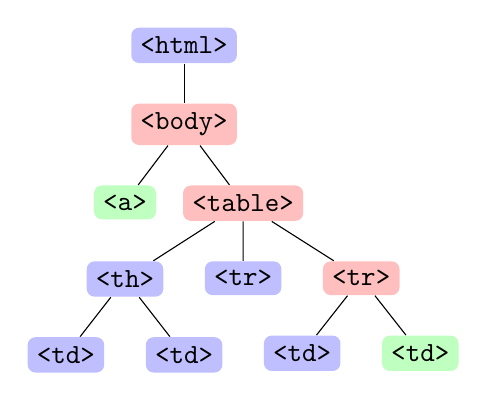
\begin{tikzpicture}[
    fact/.style={rectangle, draw=none, rounded corners=1mm,
        text centered, anchor=north, text=black, fill=blue!25},
    redcolor/.style={rectangle, draw=none, rounded corners=1mm,
        text centered, anchor=north, text=black, fill=red!25},
    greencolor/.style={rectangle, draw=none, rounded corners=1mm,
        text centered, anchor=north, text=black, fill=green!25},
    level distance=0.5cm, growth parent anchor=south]

\node (Fact01) [fact] {\texttt{<html>}} [-]
    child{
        node (kolor4) [redcolor] {\texttt{<body>}}
        child{
            node (color1) [greencolor] {\texttt{<a>}}
        }
        child{
            node (Fact04) [redcolor] {\texttt{<table>}}
            child{
                node (Fact05) [fact] {\texttt{<th>}}
                child{
                    node (fact5) [fact] {\texttt{<td>}}
                }
                child{
                    node (Fact07) [fact] {\texttt{<td>}}
                }
            }
	    child{
                node (Fact05) [fact] {\texttt{<tr>}}
	    }
            child{
                node (color3) [redcolor] {\texttt{<tr>}}
                child{
                    node (Fact10) [fact] {\texttt{<td>}}
                }
                child{
                    node (color2) [greencolor] {\texttt{<td>}}
                }
            }
        }
    }
;

\end{tikzpicture}
\end{center}
\caption{A HTML GUI model with two nodes (green) the distance will be calculated for.  The number of red nodes is the distance between the green nodes. The common anchestor is the \texttt{<body>} element.}
\label{fig:guimodeldistance}

\end{figure}
Figure \ref{fig:guimodeldistance} shows a GUI model with two elements and their common ancestor.


\subsection{Event-Task To Non-Event-Task Similarity}
It takes a bit more effort to calculate the substitution score if one task is a non-event-task.
The reason is that the non-event tasks do not represent a simple event anymore.
Therefore, they do not possess a target in the GUI.
A possible solution is to recursively visit every child of the non-event-task, gather all event tasks and then calculate the mean distance from each of those tasks to the event-task the distance shall be calculated to.
Formally, definition \ref{def:guimodeldistanceee} has to be modified so that it covers non-events as well:

\begin{definition}
%	\item Let a and b be events-tasks, then:
%\begin{equation*}d(a,b) = d(b,a) = \text{be the distance in the GUI model of the targets of event-tasks a and b.}
%\end{equation*}
	\item Let c be a non-event-task.
	\item Let E be the set containing all event-tasks that can be recursively found in c.
	\item With definition \ref{def:guimodeldistanceee} it is possible to define d as
\begin{equation*}
	d(a,c) = d(c,a) = \frac{\sum_{\forall x \in E} d(a,x)}{|E|}
\end{equation*}
\label{def:guimodeldistanceene}
\end{definition}

\subsection{Non-Event To Non-Event Similarity}
With Definition \ref{def:guimodeldistanceene} it is simple to compute the distance for two tasks since all that is to do now is to repeat the procedure of finding all event-task children of one task, calculate the distances to the other task and use the mean distances as the total distance.
The definition of d can be extended so it accepts two non-event-tasks:

\begin{definition}
	\item Let c and d be non-event-tasks.
	\item Let E be the set containing all event-tasks that can be recursively found in c.
	%\item Let F be the set containing all event-tasks that can be recursively found in d.
	\item With definition \ref{def:guimodeldistanceene} it is possible to define d as
	\begin{equation*}
		d(c,d) = d(d,c) = \frac{\sum_{\forall x \in E} d(x,d)}{|E|}
	\end{equation*}
\label{def:guimodeldistancenene}
\end{definition}
\subsection{Score}
Now that we defined the distance for three cases it is possible to compute the score $S$ of two tasks.
To transform a distance into a score we multiply all distance values with $-1$ and add a constant so that some scores are positive and some have a negative value.

\begin{definition}
	\item Let U be the set of unique tasks occurring in the user sessions.
	\item Let k be a constant that defines the maximal score.
	\item For each tupel $i,j \in U$
\begin{equation*}
		 S(i,j) = -1*d(i,j)+k
	\label{eq:subscore}
\end{equation*}
\label{def:scorewithmaximalscore}
\end{definition}
The $k$ constant should be chosen dependent on the underlying GUI model.
A large k may be chosen for very deeply, nested GUI models whereas for flat GUI models a smaller $k$ seems better.
At last this parameter has to be evaluated and carefully adjusted to the given input data.

The maximal score is reached if the distance between two elements is zero. This happens if we compare two equal elements.
A problem can occur when the score of a non-event-task to an event task is equal to maximal score.
This happens if a non-event-task has just one event-task as child and the distance of this child to the same event-task is calculated.
Since it is preferred that the score of two equal event-tasks is always larger than the score of this event-task with a non-event-task we add the penalty term $L$ to the score equation.

\begin{definition}
	\item Let E be the set of all event-tasks.
	\item Let N be the set of all non-event-tasks.
\begin{eqnarray*}
	L(i,j) &=&
	\begin{cases}
		0 & \text{if } i,j \in E \\
		\text{constant} & \text{if } i \in N \lor  j \in N\\
	\end{cases} \\
	S(i,j) &=& -1*d(i,j)+k-L
	\label{eq:subscore_adjusted}
\end{eqnarray*}
\label{def:scoreadjusted}
\end{definition}


\section{Iteration Detection And Substitution Matrix Update}
The iteration detection from Harms is also suitable for our algorithm and was not altered in any way. It reliably detects iterations and replaces them in the user sessions.
Before the sequence detection can come into play, the substitution matrix should be updated since there were new iteration tasks created during iteration detection. Those new tasks are stored in a set that contains all newly created tasks.
The update process differs just a little from the generation process with the only difference beeing that just the distances between the newly created tasks to the current set of unique tasks is as well as the distances between the newly created tasks are computed.
After the matrix has been updated, the newly created tasks are merged with the set of unique tasks and then emptied.

The update process is a very expensive procedure. An alternative to this is to set each score between an event-task to a non-event-task and therefore all scores between non-event-tasks to zero.
Both variants are evaluated in chapter \ref{chap:casestudy}.

\section{Sequence Detection}
As we figured out at the beginning of this chapter the sequence detection is the part of the algorithm that varies the most from Harms approach.
It is itself separated in four steps:
\begin{enumerate}
	\item The search for significant patterns
	\item The match retrival
	\item The task generation
	\item The sequence replacement
\end{enumerate}

\subsection{Search For Significant Patterns}
The search for significant patterns is done with an alignment method we introduced in section \ref{sec:alignments}.
The bioinformatical problem of comparing and aligning DNA/RNA/Amino acid sequences is closely related to finding more or less equal subsequences in the user sessions.
The conserved regions of biological sequences comply with those interactions that most of the users performed similarly.
We can conclude that those interactions are meaningful in the sense of fulfilling one desired task.
The goal of the alignment algorithm is now to detect the conserved regions and extract a model of the average user behaviour.
Since alignment algorithms also find approximate and not only exact similarities, this step of the sequence detection is the main difference to Harms method.

The first step of the search for significant patterns is to align every user session with any other user session with the Smith-Waterman algorithm for repeated matches.
For the rest of this section the user session will be represented by a sequence of numbers. Each number in a sequence corresponds with the unique ID of the task at this position in the user sessions.
We now describe the algignment algorithm in detail.

\subsubsection{Smith Waterman Algorithm For Repeated Matches}
The Smith-Waterman algorithm for repeated matches\cite{durbin1998} is a modified version of the original Smith-Waterman algorithm\cite{waterman1981}.
The original Smith-Waterman finds the best local similarity between two sequences.
Since we need all relevant similarities and not just the one with the best score, we define a threshold score $T$.
\begin{definition}
	Let T be the threshold score for subalignments.
	\label{def:treshold}
\end{definition}
Once a local subalignment reaches T it is considered as relevant.

We recall from the section \ref{sec:alignments} that alignment algorithms try to find the best possible score between two sequences using the underlying scoring model of substitution and gap scores.
The most na\"ive approach is to test possible combinations both sequences could be aligned. As usual, this approach is not very feasible because there are
\begin{equation*}
	\binom{2n}{n} = \frac{(2n)!}{(n!)^2} \simeq \frac{2^{2n}}{\sqrt{\pi n}}
\end{equation*}
possible global alignments of two sequences\cite{durbin1998}.
Another way would be to use some kind of heuristic but we are interested in an exact, deterministic method.
A common technique to solve this issue is dynamic programming\cite{bellman1957}.
The main idea of dynamic programming is not to calculate every possible variant but to reuse the best solutions of smaller subproblems.
This method is central to computational sequence analysis\cite{durbin1998}.

\paragraph{Basic Smith-Waterman}
The basic version of the Smith-Waterman algorithm makes use of dynamic programming by defining the dynamic programming matrix $F$ where each cell of the matrix stores the best score for aligning the elements up to the position the cell represents.
For example the cell $(2|2)$ stores the score for the best alignment of first two elements of each sequence.
Each cell is computed by getting the best score out of four choices. Prior to enlisting those, we need the following definitions:

\begin{definition}
	\item Let x,y be two sequences.
	\item Let F be a matrix with F(i,j) being the best score of aligning $x_1\dots x_i$ with $y_1\dots y_j$.
\end{definition}
Then we can compute F by repeatedly applying the following equation:
\begin{equation}
F(i,j) = max \left\{ \begin{array}{lr}0,&\\F(i-1,j-1)+S(x_i,y_j),&Substitution\\F(i-1,j)-g,&Gap\\F(i,j-1)-g.&Gap\\\end{array} \right.
\end{equation}
Figure \ref{fig:basicalignmentoperations} illustrates this formula.
The diagonal choice means we align one element from each sequence with each other.
Therefore, we have to look up the similarity of both elements in the substitution matrix.
When the score from the upper cell minus the gap penalty is bigger than the diagonal choice a gap will appear at this position in sequence y.
This is the same for when the option from the left cell is taken, just that the gap will be inserted in sequence x.
The option 0 in the equation is to prevent alignment scores to become negative.
If a match cannot be extended with its score being a positive value, it is better to start a new one later.
As we can see, it is possible to fill the whole matrix by once the trivial scores, the first row and the first column, have been initialized.

\begin{figure}
	\centering
	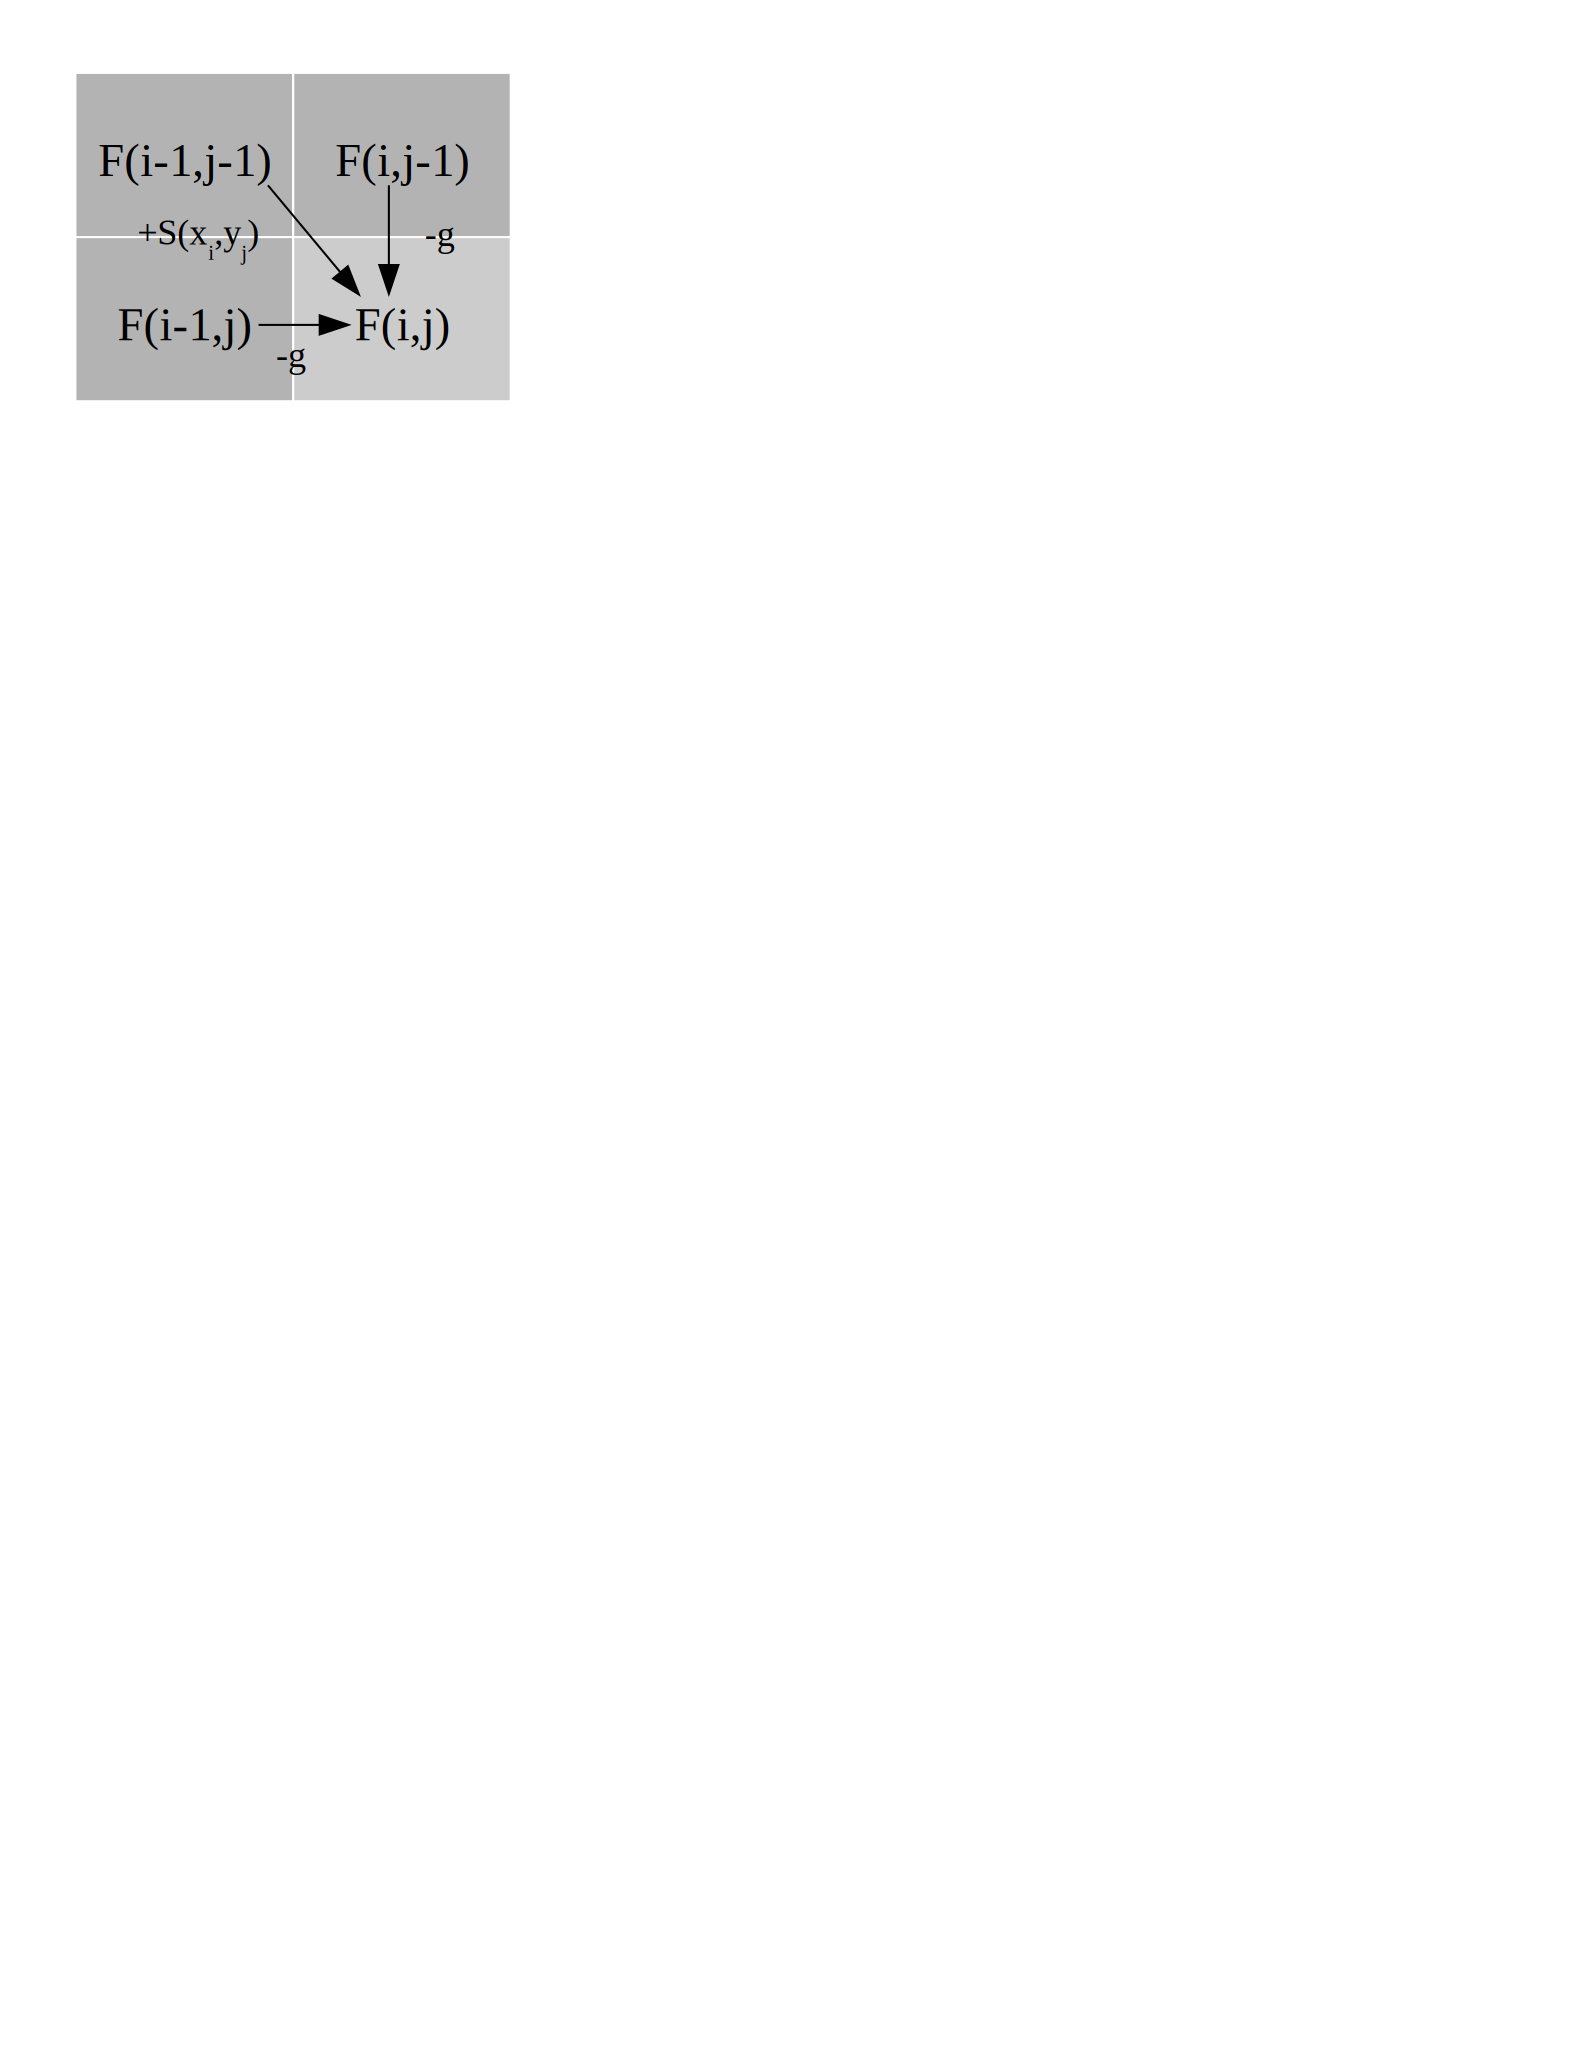
\includegraphics{img/basic_cell_fill.pdf}
	\caption{Illustration of the three operations deletion, insertion and substitution in a dynamic programming matrix.}
	\label{fig:basicalignmentoperations}
\end{figure}

\paragraph{Repeated Matches}
In the improved version of the algorithm a cell in $F$ has a slight different meaning and its computation is a bit more complex.
The first difference is that this algorithm is asymmetric in the sense of aligning sequence x to sequence y produces a different outcome than aligning sequence y to sequence x.
Hence, we define y as the pattern we want to search and x as the sequence in which we search all subsequences of y repeatedly.
This results in a final alignment where x has matched and unmatched regions.

The algorithm itself is partitioned into three parts:

\begin{itemize}
	\item Initialization
	\item Recursion
	\item Traceback
\end{itemize}

\subparagraph{Intialization}
	The initialization step is simple: \\
	Let m be the length of y

	\begin{equation*}
		F(0,j) = 0 \text{ for } j=0\dotsc m
	\end{equation*}
	This differs from the Smith-Waterman algorithm described by Durbin et al.\cite{durbin1998} who just initialize F(0,0) and do not fill the first column. There is no need to initialize the first row because a subalignment will never start with a gap. For the sake of an easy implementation it was better to initialize the first row though.

\subparagraph{Recursion}
The recursion formula for filling the matrix also has the three options for insertion, deletion and substitution as illustrated in figure \ref{fig:basicalignmentoperations}.
But as we see there are some more options.
For the first row (equation \ref{eq:firstrow}), which does not represent a real alignment of sequences but denotes the sum of completed match scores, we have two options.
The first one is to take the value from the last column so we always keep track of the total score.
This leads to the fact that the value in this line will always stay the same or increase, but never decrease.
The second choice is taken when a match reaches its maximum and has a minimum score of T.
This is the consequence of an ending match meaning this choice is just taken when we calculate the cell for an unmatched region.
To summarize the equation for the first row we can say the algorithm choses the maximum value of the last column minus T or adopts the value of the preceding cell in the first row, depending which one was larger.

Equation \ref{eq:otherrows} for the fields aside of the first row is amended by the posibility to begin its alignment score with the value standing in the first row of its own column.
Durbin et al. do not mention the fact that this makes it easier for subalignments of long sequences to reach the threshold score once a few matches have been found before.
This issue has not been investigated in this work.
The total score of the whole alignment is stored in F(i+1,0). This cell lies in an unmatched region of x and contains the sum of all completed match scores.


\begin{equation}
F(i,0) = max \left\{ \begin{array}{lr}F(i-1,0),&\\F(i-1,j)-T,& j=1,\dots,m\end{array}\right.
\label{eq:firstrow}
\end{equation}
\begin{equation}
F(i,j) = max \left\{ \begin{array}{lr}F(i,0),\\F(i-1,j-1)+S(x_i,y_i),\\F(i-1,j)-g,\\F(i,j-1)-g.\end{array}\right.
\label{eq:otherrows}
\end{equation}

\subparagraph{Traceback}
A very important point in dynamic programming algorithms is that we not just calculate and store the maximum score for each subproblem but additionally have to store which choice of the formula produced the highest value.
This makes it possible to go back from the total best score to the start and find the actual alignment of the whole sequences.
This process is called traceback.
The procedure is to go back the path that led to the final score (here in F(i+1,0)).
After going back, again take the path that led to the previous cell. Repeat this procedure until F(0,0) is reached.
Figure \ref{fig:durbindpmatrixtraceback} shows a completely filled dynamic programmic matrix and the traceback path.

\begin{figure}
\centering
\includegraphics[scale=0.4]{chapters/approach/smithwatermanrepeated.png}
\caption{Figure from Durbin et al.\cite{durbin1998}. The repeat dynamic programming matrix for two example sequences, for T = 20. Below the optimal alignment, with total score \mbox{$9 = 29-20$}. There are two separate match regions, with scores 1 and 8. Dots are used to indicate unmatched regions of x. The arrows show the traceback process, going back from the total score to the start.}
\label{fig:durbindpmatrixtraceback}
\end{figure}

\subsection{Match Retrival}
To find similar user behaviour we are only interested in the matches that reached the threshold score.
After aligning every user session with each other we extract all matches from those alignments.
We consider every subset of the alignment that is not an unmatched region as a match.
Therefore, a match consists of two sequences of numbers and can contain gaps.
We encode a gap with the value -1.
Figure \ref{fig:matchexample} shows an example of a match, containing one gap in the first sequence, two exact tasks and one substitution.

\begin{figure}[h]
	\centering
	\begin{tabular}{cccc}
		9 & 16 & -1 & 6 \\
		9 & 15 & 17 & 6
	\end{tabular}
	\caption{Example for a retrieved match. Each of the two subsequences of the sequences the match was generated from is printed in a row.}
	\label{fig:matchexample}
\end{figure}
Each of those matches is searched in all user sessions.
For this, each position in the user sessions is checked if the match in question fits at this position.
Before we can do this, we have to explain what it means that a match is found since we have to take into account how a match will be transformed into a task later.
When a match is found we store the ID of the user session it occured in as well as its position in the user session.
There are some rules that have to be fulfilled to consider a match as found:

	\begin{rules}
		\item If both elements of a position in a match are equal, this element has to be found at this position of the subsequence in which we search.
	\end{rules}
	\begin{figure}[h]
		\centering
			\begin{tabular}{cc}
				 16 & 4\\
				 16 & 4\\
			\end{tabular}
		\caption{Example for rule 1. Will only match a user session subsequence 16 4.}
		\label{fig:rule1}
	\end{figure}


	\begin{rules}
		\item If one element in a match is a gap (-1), the other element of this position is optional at this position.
	\end{rules}
	\begin{figure}[h]
		\centering
			\begin{tabular}{ccc}
				16 & -1 &6\\
				16 &  4 & 6\\
			\end{tabular}
			\caption{Example for rule 2. Will match user session subsequences 16 4 6 and 16 6.}
		\label{fig:rule2}
	\end{figure}

	\begin{rules}
	\item If both elements are not equal and the next position contains two equal elements (a) or a gap (b), either of the unequal elements can occur at this position.
	\end{rules}
	\begin{figure}[h]
		\centering
		\begin{subfigure}[b]{0.49\textwidth}
		\centering
			\begin{tabular}{cc}
				 14 & 4\\
				 16 & 4\\
			\end{tabular}
			\caption{Example for rule 3 (a). Will match 16 4 and 14 4.}
			\label{fig:rule3}
		\end{subfigure}
		\begin{subfigure}[b]{0.49\textwidth}
		\centering
			\begin{tabular}{ccc}
		\centering
				14 & -1 & 6\\
				16 & 4  & 6 \\
			\end{tabular}
			\caption{Example for rule 3 (b). Will match 16 4 6, 14 4 6, 14 6 and 16 6. }
		\end{subfigure}
		\caption{Examples for rule 3 (a) and (b).}
		\label{fig:rule3}
	\end{figure}
	\begin{rules}
	\item If both elements are not equal and the elements of the next positions are not equal as well:
		\begin{enumerate}
			\item Group all elements of one sequence together as long as the next positions still have unequal elements.
			\item A match is found if the user session matches completely one of those grouped sequences.
		\end{enumerate}
	\end{rules}
	\begin{figure}[h]
	\centering
	\begin{tabular}{ccc}
		 16 & 18 & 14 \\
		 15 & 17 & 16 \\
	\end{tabular}
	\caption{Example for rule 4. Match is found if a subsequence of a user session is 15,17,16 or 16,18,14 but not 15,18,14.}
	\label{fig:rule4}
	\end{figure}

\paragraph{Match Sorting}
Once all matches have been retrieved they have to be sorted to have an order they will be replaced in the sequences. The sorting criteria are the following:
First we sort by the number of occurence in all sequences.
The reason for this is that we want to prefer the most occurring match over all other match properties because it is likely that a task with a high occurence represents
the average user behaviour. If two matches have the same occurrence count, the length of the matches is considered. Longer matches will be replaced first.
The next two sort properties are introduced for a deterministic behaviour of the algorithm.
%The reason why is that we need an explicit order of all matches.
If two matches have the same occurrence count and the length, the sum of the user session IDs is considered and after that the sum of the task IDs.


\subsection{Task Generation}
After sorting the matches, the actual task is created from each match that has a minimum occurence of f.
This parameter is introduced to exclude those matches that just have been performed by a small number of users and therefore are not representative for a general interaction with the software.
\begin{definition}
	\item Let f be the number of occurrences a task must have in all user sessions in order to be replaced.
		\label{def:minoccurrencecount}
\end{definition}
We will now see why we had to search the matches according to the rules enlisted in the previous section. The task generation rules correspond to the search rules.
We start with an empty task of temporal relationship type \textit{sequence}.
This is the root node of the task we will convert the match to.
For this, the procedure is to evaluate each position of the match and apply some rules again.
If both elements in the match are equal, the task with this ID is added to the sequence. This is the equivalent to search rule 1.
Search rule 2 transferred to task generation leads to the creation of tasks with temporal relationship type \textit{optional}.
The created optional task has the task that is "aligned" with the gap as its child.
If the algorithm observes a position where search rule 3 is applied, a single selection with two children is created.
Both of the two unequal tasks of this position have this selection as their parent.
The adopted application of search rule 4 creates three new tasks, a selection and two sequences.
The selection is added to the root sequence, both of the sequences are children of the selection.
The sequences themselves contain the subsequent unequal tasks of one row of the match.
Figure \ref{fig:matchexampletaskgeneration} shows a match that is converted into a task. In this match all rules have been applied.

\begin{figure}[h]
	\centering
	\begin{subfigure}[c]{0.44\textwidth}
		\centering
	\begin{tabular}{cccccc}
		9 & 16 & -1 & 6 & 4& 5\\
		9 & 15 & 17 & 5 & 3& 5\\
	\end{tabular}
	\end{subfigure}
	\begin{subfigure}[c]{0.1\textwidth}
		\centering

		\Large{$\Rightarrow$}
	\end{subfigure}
	\begin{subfigure}[c]{0.44\textwidth}
		\tikzstyle{every node}=[rectangle, draw=none, rounded corners=1mm,
		        text centered, anchor=west, text=black, fill=blue!30]

		\begin{tikzpicture}[%
		  grow via three points={one child at (0.5,-0.7) and
		  two children at (0.5,-0.7) and (0.5,-1.4)},
		  edge from parent path={(\tikzparentnode.south) |- (\tikzchildnode.west)}]
		  \node {Sequence}
		  	child { node {9} }
		  	child { node {Selection}
		        	child { node {16}}
		        	child { node {15}}
		        }
		 	child [missing] {}
		 	child [missing] {}
		        child { node {Optional}
		        	child { node {17}}
		        }
		 	child [missing] {}
		        child { node {Selection}
		        	child { node {Sequence}
		        		child{node {6}}
		        		child{node {4}}
		        	}
		 		child [missing] {}
		 		child [missing] {}
		        	child{ node {Sequence}
		        		child{node {5}}
		        		child{node {3}}
		        	}
		        }
		 	child [missing] {}
		 	child [missing] {}
		       child { node {5}};

		    \end{tikzpicture}
	\end{subfigure}
	\caption{Example for task generation. The match on the left is converted into the task on the right.}
	\label{fig:matchexampletaskgeneration}
\end{figure}

\subsection{Replacement}
One last step is required to finish the sequence detection: the replacement of all generated tasks in all the user sessions.
For this we create an instance of the generated sequence and replace each subsequence in the user sessions that fits the model of the instance.
We do not need to search the positions where we can insert the instance since we stored all the occurrences in our first search.
What we have to do is to update the information about the position in all other stored match occurrence data.
For example, if we extract six task instances, match occurrences with a position after this replacement need to substract six from their start and end indices.
If a first replacement overlaps another one, the second one is ignored. Here we can see again that the order of replacement is very important  because it determines which
matches are replaced and which may be ignored.

\subsection{Repetition}
Same as in Harms et al.s approach the steps iteration detection and sequence detection are repeated until a specific condition is reached.
Harms et al. repeat until no further replacements can be made.
We propose to stop the repetition before.
Possible conditions could be that the algorithms stops once it finds less matches than a specific percentage of the number of matches that have been found in the first iteration of the algorithm.
Another possibility would be to have a fixed number of iterations.
We will evaluate those proposals in the case study section.


\clearpage
\chapter{Implementation}
\begin{itemize}
	\item Approach was implemented in Autoquest (cite)
	\item What is autoquest? Proof of concept implementation of pharms
	\item Can Process Platform indepentent, abstract events
	\item Basically just branched the autoquest-core-tasktree package
	\item Input data: User Sessions with EventTaskInstances and corresponding event Tasks
	\item Output: Generated Task Model
	\item This implementation is striclty sequential, but there is a huge potential of parallelizing sub-problems
\end{itemize}
\section{Substitution Matrix}
\subsection{Generation}
\begin{itemize}
	\item No problems for limited number of tasks
	\item For large numbers of Tasks, efficient implementation needed
	\item Implemented as Triangle Matrix of float values, stored in a single float[] (to save overhead of n*sizeof(float[])
	\item Calculation of distances between Tasks is well parallelizable, storing it to the matrix is not (yet).
\end{itemize}
\subsection{Updating}
\begin{itemize}
	\item The procedure of updating the substitution matrix is implemented but has just been tested on a very small data set. 
	\item Since the Matrix grows with O(n*(n+1)/2), for large data sets the calculation of non EventTasks is switched off, because each generated tasks increases n.
	\item Also, the computation of non-EventTasks is complex itself. First, for each Task all EventTasks have to be searched (done via visitor pattern). 
	\item Then for each found EventTasks, distances have to be calculated (or read from Substitution Matrix)
	\item THis process could as well be parallelized, still, storing in the matrix has to be synchronous. Also, when the matrix is updated, it's size has to be enlarged. The problem with this is, that then a data structure with a dynamic size has to be used, which itself is not very memory efficient. 
	\item A solution is to allocate a very large matrix from start and for increasing allocate an even larger matrix and copy the old matrix to the new. This procedure has a high peak memory usage but will reduce mean memory usage of the object distribution matrix (Numbers of the sizes of Float, ArrayList<Float> and float[] here)
\end{itemize}

\section{Alignments, Match Count, and Sorting}
\begin{itemize}
	\item Both the pairwise alignment of each of the sessions and the occurence count are actions that have been implemented as parallel algorithms
	\item Huge speedup possible, still very time and ram consuming on large datasets
	\item The Results of the match count has to be sorted
\end{itemize}

\section{Replacment}
\begin{itemize}
	\item Replacment is so far strictly serial, but is parallelizable. For each user session a datastructure is kept, which replacements have been performed on it. 
	\item This datastructure requires synchronized access of the threads
\end{itemize}



\clearpage
\chapter{Case Study}
To validate our method, we run the alignment approach of task tree generation against the same case study as Harms et al. did.
The user traces were collected on an application portal of the university.
Figure \ref{fig:screenshotmasterportal} shows a screenshot of the first page of the portal.
After logging in, users can fill out multiple forms regarding their personal data as well as upload their CVs.
In this case study 555 user created arround 3602 appropriate user sessions.
Further details about the data are enlisted in table \ref{tab:casestudy2}.
The data of the traces is XML structured. 
Figure \ref{fig:xml} shows the format of one \textit{onclick} event. 
%After reading in the input files event tasks for each event are created.
\begin{figure}[h]
	\includegraphics[width=\textwidth]{chapters/casestudy/masterportalscreenshot.png}
	\caption{Screenshot of the website the data was collected with.}
	\label{fig:screenshotmasterportal}
\end{figure}
\begin{figure}
\begin{verbatim}
<event type="onclick">
      <param name="timestamp" value="1389109340615"/>
      <param name="target" value="DSuS8oahm5 ... NfhupVDJCn=="/>
      <param name="Y" value="64"/>
      <param name="X" value="662"/>
</event>
\end{verbatim}
\caption{Example of one event in XML structure.}
\label{fig:xml}
\end{figure}

\begin{table}
	\centering
	\begin{tabular}{c r r}
		\toprule
		\multirow{5}{*}{\textbf{Date, Users \& Sessions}} & Start of Recording & 25 October 2013 \\
		      & End of Recording & 7 March 2014 \\
		      & Recorded Users & 555 \\
		      & Recorded User Sessions & 4,129 \\
		      & Considered User Sessions & 3,602 \\
		\midrule
		\multirow{6}{*}{\textbf{Events}} & Recorded Events & 350,368 \\
		      & Relevant Events & 306,568 \\
		      & Double Clicks & 6,437 \\
		      & Focus Changes & 89,825 \\
			   & Considered Events & 210,306 \\
			   & Different Events & 1,897 \\
		\bottomrule
	\end{tabular}
	\caption{Case study overview.}
	\label{tab:casestudy2}
\end{table}

We are interested in several aspects of the task tree creation with the alignment approach.
First of all, we want to examine the necessity of the calculation of the distance between non-event-tasks.
The calculations of those distances are very expensive operations so we want to know if this step could be left out and we still find approximately the same amount of tasks in the same quality.
After that, we study the algorithms termination conditions with the goal to find out if we can terminate the algorithm earlier than proposed in chapter \ref{chap:approach}.

Afterwards, we evaluate the performance of the alignment approach and compare it to the performance of the n-gram approach.
At last, we discuss the created task tree by means of representative task examples after running the alignment approach on the full case study.
All experiments were executed on an AMD Opteron(TM) Processor 6276 (64 core) with 250GB of ram after we figured out that an Intel(R) Core(TM) i5-2520M CPU @ 2.50GHz with 8GB of ram is not sufficient to run the alignment approach on large numbers of user sessions.
The Java virtual machine was started with the following parameters:
\begin{itemize}
	\item -XX:+UseConcMarkSweepGC
	\item -Xmx84000m
\end{itemize}

\section{Parameters}
The alignment approach has several parameters that have to be set before running the algorithm. Some values of the parameters may also depend on the underlying data.
All parameters are described in the approach chapter. Table \ref{tab:parameters} gives a short summary of all available parameters that can be set and also the values
we used in this case study. Those parameters were manually chosen by trial and error and do not guarantee the best possible results.

\begin{table}
	\begin{tabularx}{\textwidth}{ r X r r}
% \renewcommand{\arraystretch}{1.5}
	   \toprule
		\multirow{2}{*}{\textbf{Parameter}} & \multirow{2}{*}{\textbf{Function}} & \multirow{2}{*}{\textbf{Definition}} & \textbf{Value in} \\
		& & &\textbf{case study}\\
	     \midrule
	       \emph{k} & The value of the maximum score in the substitution matrix& \ref{def:scorewithmaximalscore}& 6  \\
			 \noalign{\medskip}
	       \emph{L} & Penalty for the score between non-event-tasks & \ref{def:scoreadjusted} & 3 \\
	      \noalign{\medskip}
			 \emph{T} & Threshold score for determination of match importance & \ref{def:treshold} & 9\\
	      \noalign{\medskip}
			\emph{g} & Gap penalty for inserting gaps & \ref{def:gappenalty} & 3 \\
	      \noalign{\medskip}
			 \emph{f} & Number of occurrences a task must at least have in all user sessions to be replaced & \ref{def:minoccurrencecount} &3\\
	       \bottomrule
 \end{tabularx}
 \caption{Table of all parameters of the alignment approach that can be adjusted for the task tree generation.}
 \label{tab:parameters}
 \end{table}


\section{Data Preprocessing}
After loading the input data from all XML files the following preprocessing steps are performed. The information about each command is copied from its manual page in AutoQUEST. 
The goal of the preprocessing is to fix several flaws the input data has.
\begin{description}
	\item[condenseHTMLGUIModel]\hfill\\ Merges all equal nodes in the GUI-Model.
	\item[condenseMouseClicks]\hfill\\ Reduces a sequence of mouse button down, mouse button up and mouse click with the same button on the same event target to a single mouse click with that button on that target. The mouse button down and mouse button up events are discarded.
	\item[correctKeyInteractionTargets]\hfill\\ Iterates the provided sequences and sets the target of all key interaction events to the GUI element having the current keyboard focus. The current keyboard focus is determined either by keyboard focus events or by using the target of the first key interaction in a sequence. Events changing the keyboard focus are discarded herewith.
	\item[correctTabKeyNavigationOrder]\hfill\\ Iterates the provided sequences and corrects the order of events in case of tab key navigation. This is required, as from time to time the event of pressing the tab key for navigation in formulars comes before the text input event in a text input field out of which the tab key navigates.
\end{description}

\section{Calculation Of Distances Between Non-Event-Tasks}
\label{sec:noneventtasks}
In this section we investigate if the calculation between non-event-tasks is neccessary by comparing the two generated task trees, one with the additional calculations and one where
we set every score involving a non-event-task to zero. 
Table \ref{tab:resultsnoneventtasks} shows the results of this experiment.
The calculation of distances between non-event-tasks is not an issue on very small subsets (ca. 40 user sessions) of the case study. 
But once we include more sequences the index for the array we use for storing the scores in the substitution matrix hit the limit of \texttt{Integer.MAX\_VALUE}.
A possible solution for this issue is not to calculate the distances between the non-event-tasks and thus saving computation time and memory usage.
The number of found tasks is significantly higher when the distances between non-event-tasks are calculated but the drawback is that the time to generate the task tree increases drastically as well.
The quality of the generated task trees also differs.
One criterion of the quality of task trees is the depth. 
Each level in a task tree increases the depth by one.
Without the calculated distances the generated task trees have a flatter structure (maximum depth is 6 with calculated distances, 4 without).
This flat structure can be explained by the reduced number of repetitions of the algorithm because we hit the termination condition earlier in the algorithm.
An early stop decreases the possibility of inserting new levels into the tasks.

With the calculation of the distances long interactions like login or account creation procedures can be found.
Those long tasks do not always represent correct user interactions.
Figure \ref{fig:noneventaccountcreation} shows a task tree for the first part of the account creation process.
We can see several subtasks of the task where the subtask does not model user behaviour correctly.
\texttt{Selection 2691} followed by \texttt{optionality 2692} makes no sense since the text input of the optionality should just happen after the text input field has been clicked on.
This happens in \texttt{iteration 1288}, the first child of \texttt{selection 2691}. 
The optionality with the text input should actually be in a sequence with \texttt{iteration 1288} as its preceeding element.
Another part of the task tree that represents no real user behaviour in this example task is \texttt{sequence 1656}.
The first selection in it gives the possibility to either click or double click on an input field.
While double clicking a text field is not an effective behaviour of a user, it is still a valid action to achieve his goal to enter his email address.
The meaningless part is the text input on the email input field, followed by the same event again. This should either be just one event at all or be found in an iteration.
There are several more examples where the non-event-task distance calculation did not improve the task tree quality.
In summary, the amount of tasks created but not their quality can be increased by enabling the distance computing.

With the large increase of computational time and the integer limitation of the Java array indexes in mind we will set the score to or from non-event-tasks to zero in all further experiments.
The reason for this is that we have an increase in time by over 3800\% even in this very small example and we cannot asume a linear scaling of this increase because nearly all algorithms we use have a complexity of $O(n^2)$.
A parallel computation of the distances and a clever storage of all already calculated values could as well fix this issue but this could not be addressed in this thesis due to time issues.

\begin{figure}[h]
	\centering
	%\includegraphics[scale=0.7]{chapters/casestudy/noneventcreateaccount.png}
	\includegraphics[scale=0.75]{chapters/casestudy/noneventcreateaccount.png}
	\caption{An example for a task found by alignment task tree generation with distance calculation between non-event-tasks.}
	\label{fig:noneventaccountcreation}
\end{figure}

\begin{table}[h]
	\centering
	\begin{tabular}{l r r}
		\toprule
		&  \multicolumn{2}{c}{\textbf{Testcase}} \\
		\cmidrule{2-3}
		\textbf{Type of non-event-task}& \textbf{with distances}& \textbf{without distances} \\
		\midrule
		Sequences & 352 & 50 \\
		Iterations& 38  & 38 \\
		Selections& 328 & 21 \\
		Optionals & 6   & 8  \\
		\midrule
		\textbf{Performance indicator} & \\
		\midrule
		Time (s)     & 72.2 & 1.9 \\
		Number of repetitions & 35 & 7\\
		\bottomrule
	\end{tabular}
	\caption{Results of the version with and without calculation of the distances between non-event-tasks}
	\label{tab:resultsnoneventtasks}
\end{table}

\section{Evaluation Of Termination Conditions}
In this section we will investigate if the algorithm for the task tree generation can be terminated with other conditions than the condition mentioned in chapter \ref{chap:approach}.
The described behaviour is that the algorithm stops if no further replacements could be performed.
It has been observed that the most matches are found in the first few repetitions of the sequence detection phase.
Table \ref{tab:timesandmatchesperiteration} and the corresponding figure \ref{fig:hasehase} supports this claim. We can see that the number of matches found in each repetition decreases rapidly.
After the 6th repetition we detect 0.01\% of the matches found in the first sequence detection. We could stop the algorithm here. But since the algorithm finishes shortly after (after the 10th repetiton),
we keep the termination condition for this case study as it is defined in the approach.
If on other case studies the algorithm repeats more often, it can be considered to change the termination condition to a fixed number of iteration.
Another propable condition is to stop when the number of found matches falls below a fraction from the matches found in the first repetition.

As we see in section \ref{sec:noneventtasks} the number of iterations drastically increases if the distances between non-event-tasks are calculated.
If a good solution for the large computation time of the distances is found, this would be a possible use case of a different termination condition.

\begin{table}[h!]
		\centering
	\begin{tabular}{ l r r r }
		  \toprule
			& & \multicolumn{2}{c}{\textbf{Time (m)}} \\
			\cmidrule{3-4}
		  \textbf{Repetition No.} & \textbf{Matches} & \textbf{Absolute}& \textbf{Relative} \\
		  \midrule
     		    0  & 1,112,794 & 26.17 & 26.17\\
	            1  & 381,190   & 39.16 & 12.99\\
		    2  & 167,677   & 45.52 & 6.36\\
		    3  & 63,964    & 51.00 & 5.48\\
		    4  & 26,171    & 55.83 & 4.83\\
		    5  & 12,627    & 60.72 & 4.89\\
		    6  & 8,660     & 65.48 & 4.76\\
		    7  & 7,517     & 70.34 & 4.86\\
		    8  & 7,232     & 75.02 & 4.68\\
		    9  & 7,214     & 79.74 & 4.72\\
		    10 & 7,214     & 84.49 & 4.75\\
		  \bottomrule
		   \end{tabular}
		   \caption{Matches found per repetition and the time for each repetition. All times in minutes.}
		   \label{tab:timesandmatchesperiteration} %TODO labelanpassen -> repetition
	\end{table}
	\begin{figure}[h!]
		\centering
		\includegraphics[]{chapters/casestudy/hasehase.pdf}
		\caption{Graph with matches found per repetition and the time per repetition.}
		\label{fig:hasehase}
	\end{figure}


\section{Performance Evaluation}
To evaluate the performance of both the alignment approach and the n-gram approach we run each task tree generation algorithms against different sized subsets of the case study.
We chose user session sets with the size of 10, 100, 1000 and the full case study. Figure \ref{fig:performance} and table \ref{tab:comparisontasktreegenerations} show the results of this experiment.
We can see that the alignment approach is slower on any size of input data.
But with the increasing number of user sessions we can observe that the computation time increases notebly.
As a side note the memory consumption of the alignment approach for the full case study was 46.9GB at its maximum.
The n-gram approach used 1.3GB memory for the same data set.
The memory usage of the other data set sizes were not tracked.
In summary the alignment approach is definitely more resource intensive than the n-gram approach.
\begin{table}[h]
	\centering
	\begin{tabular}{ r r r }
		\toprule
		& \multicolumn{2}{c}{\textbf{Execution time (s)}} \\
		\cmidrule{2-3}
		\textbf{Number of user sessions} & \textbf{n-gram approach} & \textbf{alignment approach} \\
		\midrule
		10 	& 2.655	& 3.141 $\simeq \pi$ \\
		100 	& 5.681	& 12.019\\
		1000 	& 60.775	& 419.063\\
		\midrule
		3602 	& 1,417.370 & 5,780.050\\
		\bottomrule
	\end{tabular}
	\caption{Comparison between execution times (seconds) of n-gram approach and alignment supported task tree generation.}
	\label{tab:comparisontasktreegenerations}
\end{table}


 \begin{figure}[h]
	\centering
	\includegraphics[]{chapters/casestudy/performance.pdf}
	\caption{Scaling behaviour of both approaches.}
	\label{fig:performance}
\end{figure}


\section{Generated Task Trees}
In this section we analyse the tasks we generated with the alignment approach. 
We were able to create tasks that describe effective user behaviour but also could find examples for wrong tasks.
With wrong tasks we mean tasks that allow actions that are either not possible on the underlying GUI-model or make no sense.
The quantity of created tasks can be found in table \ref{tab:taskquantity}. 
We find around 6000 tasks less than Harms et al. but are able to create tasks of temporal relationship type \textit{selection} and \textit{optional}.

\begin{table}
	\centering
	\begin{tabular}{ r r r }
	   \toprule
	    & \multicolumn{2}{c}{\textbf{Number of tasks}} \\
		\cmidrule{2-3}
		\textbf{Type of task}& \textbf{n-gram approach} & \textbf{alignment approach} \\
	   \midrule
	   All non-event-tasks 	& 10,634 			& 4,635 \\
		\midrule
	   Sequences 				& 9,530 				& 2,759 \\
	   Iterations 				& 1,104 				& 619 \\
	   Selections 				& -\hspace{12pt}	& 1,156 \\
	   Optionals 				& -\hspace{12pt} 	& 101 \\
	   \bottomrule
\end{tabular}
\caption{Comparison of the n-gram approach from Harms et al. and the alignment approach. The alignment approach finds less task but is able to detect selections and optionals.}
\label{tab:taskquantity}
\end{table}

The created tasks differ in quality as well. 
Figure \ref{fig:mixedtasktree} shows a task tree that constists of two different interactions: A login and a password reset.
The task starts with the tab key pressed on a textfield that is for entering user names. 
We can see that the actual entering of the username follows at the end of this task tree. 
First, the textfield for the user name is clicked on in \texttt{iteration 210306} and then input is entered in \texttt{iteration 210312}. 
The task tree should have \texttt{iteration 210306} as the first element in \texttt{sequence 2098703}.
The wrong order of some interactions can be observed in other example, too.  

Another notable point in this task tree is that it combines two different user interactions. 
The input of the email address is a text input field of the page where users can reset their password while the login button allows users to enter the personal area 
after entering their credentials. It is not correct to merge both tasks into one task tree since they are on different pages.
The alignment approach identifies the different actions correctly as a selection (\texttt{selection 2098704}) though. 

\begin{figure}[h]
	\centering
	\includegraphics[scale=0.75]{chapters/casestudy/mixedtasktree.png}
	\caption{Example for a task tree consisting of two different interactions made by the user.}
	\label{fig:mixedtasktree}
\end{figure}

The alignment approach for task tree generation creates tasks like shown in figure \ref{fig:preprocessing_needed}.
It is basically a selection of two sequences, each sequence has two event-tasks. 
The order of the event-tasks in one sequence is reversed in the other sequence.
We find numerous tasks of this kind.
The main issue with tasks like this is that a \texttt{ValueSelection} on an \texttt{input\_checkbox} and a click on this checkbox are just one action by the user but two events are created for this action.
This task is an example for the necessity of further preprocessing of the input data. 
Similar as in the \texttt{condenseMouseClicks} preprocessing command, all clicks on an \texttt{input\_checkbox} before or after a value selection should be discarded.

\begin{figure}[h]
	\centering
	\includegraphics[scale=0.75]{chapters/casestudy/preprocessing_needed.png}
	\caption{Example for a created task that shows that further data preprocessing is required.}
	\label{fig:preprocessing_needed}
\end{figure}
The last issue we address in this section is the missing detection and merging of similar or equal tasks.
Figure \ref{fig:newpassword} and figure \ref{fig:newpassword-1} both describe the same user interaction of setting a new password. 
The tasks themselves represent correct user behaviour and are positive examples for tasks generated by the alignment approach.
The only difference is the order of the children in \texttt{selection 2611158}. 
But since the order in a selection does not matter, both generated task trees are semantically equal.
\begin{figure}
	\centering
	\includegraphics[scale=0.75]{chapters/casestudy/newpassword.png}
	\caption{Example for a task for setting a new password (Version 1).}
	\label{fig:newpassword}
\end{figure}
\begin{figure}
	\centering
	\includegraphics[scale=0.75]{chapters/casestudy/newpassword-1.png}
	\caption{Example for a task for setting a new password (Version 2).}
	\label{fig:newpassword-1}
\end{figure}

\section{Discussion}
The results of all experiments show that the alignment approach still has to cope with some problems.
First of all, the performance and resource usage are a downside of this approach. 
The alignment version of autoquest is no longer able to run its task tree generation on common bulk hardware. 
Even on a server with 64 processors and a large amount of memory our approach is still slower than the n-gram approach implementation, which does not use any parallelisation.
When calculating distances between non-event-tasks the expected performance is even worse, although it may be worthy calculating those.

Another point is that the alignment approach is not able to identify and merge similar tasks. 
This problem has also not been solved by Harms at al. yet. 
There are several ways or metrics on how to determine if two tasks are equal.
For example we could calculate the Levenshtein distance of two tasks. 
The calculation of Levenshtein distance is very similar to the Needleman-Wunsch and Smith-Waterman algorithm. 
It uses a very simple scoring scheme as it just counts the number of insertions, deletions or mismatches between two sequences.
Once two equal tasks are found they should be merged. 
We do not propose an algorithm for merging tasks in this work.

In our case study we also detected that more preprocessing of the input is needed in some cases in order to generate better task trees.
Clicks on an \texttt{input\_checkbox} before or after a \texttt{ValueSelection} should always be discarded. 
Further research is needed to find other similar necessary preprocessing steps. 
An imaginable preprocessing function could be to remove clicks on radio button, too if \texttt{ValueSelections} on that radio button pre- or succeed the click.

The last problem we discuss in this section is the wrong order of tasks in a task tree and its consequence of incomplete task trees.
The task trees we generate are highly dependent on the scores we assign to different components such as substitution matrix and the gap penalty.
The scores we calculate for substitutions in our substitution matrix are just one possibility of a metric of task similarity. 
The distance in a GUI-Model is a good start to find similar or related tasks but may not be sufficient to completely model user interactions on specific graphical user interfaces.
Further research is needed to improve the scoring for substitutions. 
For example, it could be possible to manually create a database of tasks that are usually related to each other.
This database could be used to add more knowledge to the substitution matrix.

It is also interesting to find improvements for the values of the gap penalty, the maximal score of the substitution matrix and the alignment threshold score.
Further research could focus on finding an optimal combination of all parameters to improve the amount and the quality of the generated task trees.





\clearpage
\chapter{Discussion}
\begin{itemize}
	\item Hard to compare tasktrees, theres no general measurement for it.
	\item Generated task trees can represent user behaviour
	\item This method is resource and time consuming 
\end{itemize}
%Fact: We can't compare task trees in general


\chapter{Conclusion}
With the alignment approach for sequence detection we created a valuable framework for task tree generation. 






%\section{Perspective}
%\input{}

%\section{Summary}
%\input{./}

\clearpage
\addcontentsline{toc}{section}{Literature}
\bibliographystyle{apalike}
\bibliography{literature}



\end{document}
